% By zmienic jezyk na angielski/polski, dodaj opcje do klasy english lub polish
\documentclass[polish, 12pt]{aghthesis}
\usepackage{babel}
\usepackage[utf8]{inputenc}
\usepackage{url}
\usepackage{indentfirst}
\usepackage{amsmath}
\usepackage{comment}

\author{Dawid Romanowski, Wojciech Czarny}

\title{Implementacja metody SPH \\ na procesory graficzne}

\supervisor{dr hab.\ inż.\ Krzysztof Boryczko, prof.\ nadzw.\ AGH}

\date{2014}

% Szablon przystosowany jest do druku dwustronnego, 
\begin{document}
\maketitle{}
\tableofcontents
\clearpage


\section{Opis problemu}

	Symulacja czasu rzeczywistego zjawisk fizycznych jest zagadnieniem złożonym zarówno od strony teoretycznej jak i od strony implementacyjnej. Aby uzyskać realistycznie wyglądający efekt wymagane jest opracowanie szczegółowego modelu fizycznego danego zjawiska, zapisanie go w taki sposób aby umożliwić jego implementację i na końcu olbrzymia moc obliczeniowa, aby móc podziwiać efekty działania modelu w czasie rzeczywistym. Pierwsze dwa kroki są zależne od nas i możemy je do woli szlifować, jednak w obliczu zbyt małej mocy procesorów jedyny możliwy efekt końcowy to zbiór danych wyjściowych otrzymywany po wykonaniu wszystkich obliczeń - rzecz bezużyteczna w symulacjach czasu rzeczywistego takich jak na przykład gry komputerowe.

	W symulacji zjawisk fizycznych często występuje konieczność wykonywania dużej ilości prostych, powtarzalnych obliczeń dla różnych elementów układu. Przykładem może być symulacja zachowania żdźbeł trawy w szerokim polu. Mogą być ich miliony, a dla każdego z nich musimy wykonać podobne obliczenia zależne od takich czynników jak kierunek wiatru, nacisk otaczających elementów czy ukształtowanie podłoża. CPU nie będzie w stanie nadążyć przy tak olbrzymiej liczbie elementów nawet jeśli odpowienio wykorzystamy wszystkie dostępne rdzenie. 
	

		Gdy procesory przestały znacząco zwiększać swoją prędkość taktowania, a zaczęła rosnąć ich koegzystentna ilość, popularniejsze stało się przeprowadzanie niezależnych, zrównoleglonych obliczeń w celu pełnego wykorzystania potencjału sprzętu. GPGPU (general purpose computation on graphics processing unit) to technika wykonywania równoległych obliczeń na procesorach graficznych, która zyskuje na popularnośći w ostatnich latach. Wynika to z tego, że w nowoczesnych GPU wykorzystywany jest model obliczeniowy SIMT (single instruction, multiple threads), który w połączeniu z ogromną (w stosunku do CPU) ilością rdzeni (setki, czy nawet tysiące) sprawia, że implementacje pewnych algorytmów mogą uzyskać olbrzymie przyspieszenie.

	Zjawisko fizyczne, które będzie nas interesować w naszej pracy to zachowanie cieczy znajdującej się za tamą w zamkniętym zbiorniku, w przypadku przerwania tejże tamy i wylewania się cieczy do zbiornika. W przypadku symulacji zachowania płynów nie jest możliwa wizualizacja wyników w czasie wykonywania obliczeń, gdy obliczenia uwzględniają wszystkie oddziaływania pomiędzy elementami modelu fizycznego. Konieczna jest zatem dyskretyzacja problemu oraz przyjęcie uproszczonych zjawisk lub zastąpienie ich prostszymi rozwiązaniami aproksymującymi ich zachowania. Istnieje wiele metod symulowania cieczy - DPD (dissipative particle dynamics), SPH (smoothed particle hydrodynamics) czy SDPD (smoothed dissipative particle dynamics), każda mająca swoje zalety i wady.

	Zadaniem naszej pracy jest implementacja metody SPH w technice GPGPU oraz stworzenie aplikacji, która umożliwi wizualizację zachowania cieczy w trakcie wykonywania symulacji przerwania tamy. Pomimo iż metoda ta została pierwszy raz zaproponowana w roku 1977, to dopiero od niedawna możliwe jest jej wykorzystanie do zaprezentowania wyników w czasie rzeczywistym.

\subsection{Opis użytkownika}
	
	Realizacja pracy zakłada istnienie dwóch rodzajów użytkowników.
	
	Pierwszym i najważniejszym jest osoba chcąca osiągnąć te same cele, których realizacji podjęli się autorzy pracy. Dla tego użytkownika zaimplementowany system oraz dokumentacja projektu są zbiorem przemyśleń i wskazówek do odtworzenia i rozwoju powstałej technologii.
	
	Drugim typem użytkownika jest osoba korzystająca z zaimplementowanego systemu w celu zobaczenia jego możliwości oraz lepszego zrozumienia metody hydrodynamiki cząstek wygładzanych poprzez manipulację parametrów układu przy użyciu interfejsu użytkownika, oraz obserwację wpływu dokonywanych zmian dzięki modułowi graficznemu aplikacji.
	
\section{Opis metody SPH}
\subsection{Wstęp}
			
			Metoda Smoothed Particle Hydrodynamics (SPH) początkowo miała służyć do symulacji zjawisk astrofizycznych takich jak powstawanie galaktyk czy gwiazd. Zaproponowana niezależnie w 1977 roku prez Ginolda i Monaghana oraz Lucy obecnie jest często wykorzystywana do symulacji zjawisk w mniejszej skali - w szczególności zachowań płynów. 

			Ideą tej metody jest wyróżnienie pewnego dyskretnego zbioru węzłów (zwanych dalej cząstkami) badanego przez nas płynu, nadanie im pewnych własności fizycznych a następnie interpolacja tych własności fizycznych w pewnej przestrzeni. Do interpolacji wykorzystywane są funkcje wygładzające, które zamieniają punktową reprezentację wartości fizycznych na reprezentację przestrzenną.

			SPH jest metodą Langrange'owską z czego wynika, że cząski mogą się poruszać w czasie. W naszym modelu ograniczyliśmy się do trzech rodzajów sił działających na cząstki. Siła grawitacyjna, siła spowodowana różnicą ciśnień oraz lepkość.

		\subsection{Równanie Naviera-Stokesa}

			Metoda SPH jest oparta na równaniu hydrodynamicznym Naviera-Stokesa

			\[{\rho}[\frac{\partial v}{\partial t} + v \cdot \nabla v ]= F - \nabla p + \mu \nabla^2 v \label{eq:navier-stokes} \tag{1}\]

			\[{\rho}(\nabla \cdot v)=0 \label{eq:continuity} \tag{2}\]

			dla cieczy nieściśliwych, gdzie: ${\rho}$ to gęstość cieczy, ${\mu}$ to współczynnik lepkości a F reprezentuje zewnętrzne siły działające na ciecz.
			
			Analiza równania (\ref{eq:navier-stokes}) pokazuję, że przyspieszenie jest zależne jedynie od sił zewnętrznych działających na cząstkę, ujemnego gradientu ciśnienia układu oraz lepkości cieczy. Jedyna siła zewnętrzna, która interesuje nas w naszej pracy to siła grawitacji. Możemy więc zapisać: \[F={\rho}g \label {eq:gravity_force} \tag{3} \] Czynnik $v {\cdot} {\nabla} v$ reprezentuje przyspieszenie konwekcyjne, które jest efektem niezależnego od czasu przyspieszenia cząstek w zależności od przestrzeni. $-{\nabla}$p oznacza, że ciecz będzie się poruszać z przestrzeni o większym ciśnieniu w kierunku mniejszego ciśnienia. Lepkość reprezentowana jest jako stała lepkości razy laplasjan pola prędkości, który można interpretować jako różnicę między prędkością w danym punkcie a średnią prękością w małej otaczającej go przestrzeni. Lepkościa rozprasza pęd czątek i sprawia, że układ dąży do stanu równowagi.
			
			Równanie (\ref{eq:continuity}) jest po prostu równaniem zachowania masy. W naszej pracy nie było ono istotne ze względu na cechy metody SPH, które gwarantują, że jest ono spełnione w każdej sytuacji.
			 
		\subsection{Funkcje wygładzające}
			
			Celem funkcji wygładzającej jest transformacja reprezentacji cząstki z punktowej masy na przestrzenną. Funkcje wygładzające najczęściej przyjmują kształt zbliżony do rozkładu normalnego, należą conajmniej do klasy ${C^2}$ (mają ciągłą pierwsza i drugą pochodną) i są znormalizowane (całkują się do 1 od $-{\infty}$ do $+{\infty}$). Prostym przykładem takiej funkcji może być funkcja Gaussa \[W_G(r,h)=\frac{1}{h^{\nu}\pi^{{\nu}/2}}exp(-\frac{r^2}{h^2}) \label{eq:gaussian} \tag{4}\] gdzie ${\nu}$ to ilość wymiarów, r to odległość od od cząstki której estymujemy wielkość fizyczną i h to tak zwany promień wygładzania.
			
			Mając tak zdefiniowany promień wygładzania oraz dowolną dyskretną dystrybucję czątek, możemy estymować wartość fizyczną A w dowolnym punkcie przestrzeni i jako: \[{A}_i=\sum_{j=1}^{N}m_j\frac{A_j}{\rho_j}W(r_{ij},h_j) \label{eq:calc_all} \tag{5}\] gdzie ${r_{ij}}$ to odległość od cząstki j do punktu w przestrzeni, który rozważamy (pozycja i), ${m_j}$ to masa cząstki j, ${h_j}$ to promień wygładzania cząstki j, a suma jest po wszystkich cząstkach ze zbioru. 
			
			
			Przy doborze odpowiedniej funkcji wygładzającej W kluczową rolę odgrywa promień wygładzania h. Funkcja Gaussa nie jest używana do obliczeń ponieważ fakt, iż dąży ona do 0 w nieskończoności - rozciąga się w nieskończoność. Korzystając z niej, wszystkie cząstki brałyby udział przy obliczeniach w każdym punkcie. Jest to niepotrzebne, szczególnie kiedy cząstka jest bardzo odległa od rozpatrywanego punktu. Dlatego przeważanie dobiera się takie funkcje wygładzające, że dla ${r_{ij} > h}$ wartość funkcji wynosi 0. Przykładem takiej funkcji może być
			
			\[ W_{ij} = \frac{1}{\pi h^3} \left\{ 
				\begin{array}{l l l}
					1 - \frac{3}{2}(\frac{|r_{ij}|}{h})^2 + \frac{3}{4}(\frac{|r_{ij}|}{h})^3  & \quad \text{gdy ${0 \leq \frac{|r_{ij}|}{h} < 1}$}  \\ 
					\frac{1}{4}[2 - (\frac{|r_{ij}|}{h})]^3  & \quad \text{gdy ${1 \leq \frac{|r_{ij}|}{h} < 2}$}  \\ 
					0 & \quad \text{gdy ${\frac{|r_{ij}|}{h} \geq 2 }$} 
				\end{array} \right.\ \label{eq:kernel_function} \tag{6}\]
			\ \\
			zaproponowana przez Monaghana i Lattanzio w \cite{MonLat} czy:
			
			\[ W_{ij} = \left\{
				\begin{array}{l l}
					\frac{105}{16 \pi h^5}(1 + 3 \frac{|r_{ij}|}{h})(1-\frac{|r_{ij}|}{h})^3 & \quad \text{gdy ${|r_{ij}| \leq h}$}  \\ 0 & \quad \text{gdy ${|r_{ij}| > h}$} 
				\end{array} \right.\ \label{eq:kernel_function} \tag{7}\]
			\ \\
			opisywana w pozycji \cite{Lucy}
			
			My zdecydowaliśmy się wykorzystać drugą opcję, głównie ze względu na łątwiejszą implementację. 
			
			Kolejnym problemem przy doborze odpowiedniego promienia wygładzania jest to, zbyt duża lub zbyt mała wielkość może całkowicie zaburzyć wyniki eksperymentu.
			\begin{figure}[h!]
			\centering
			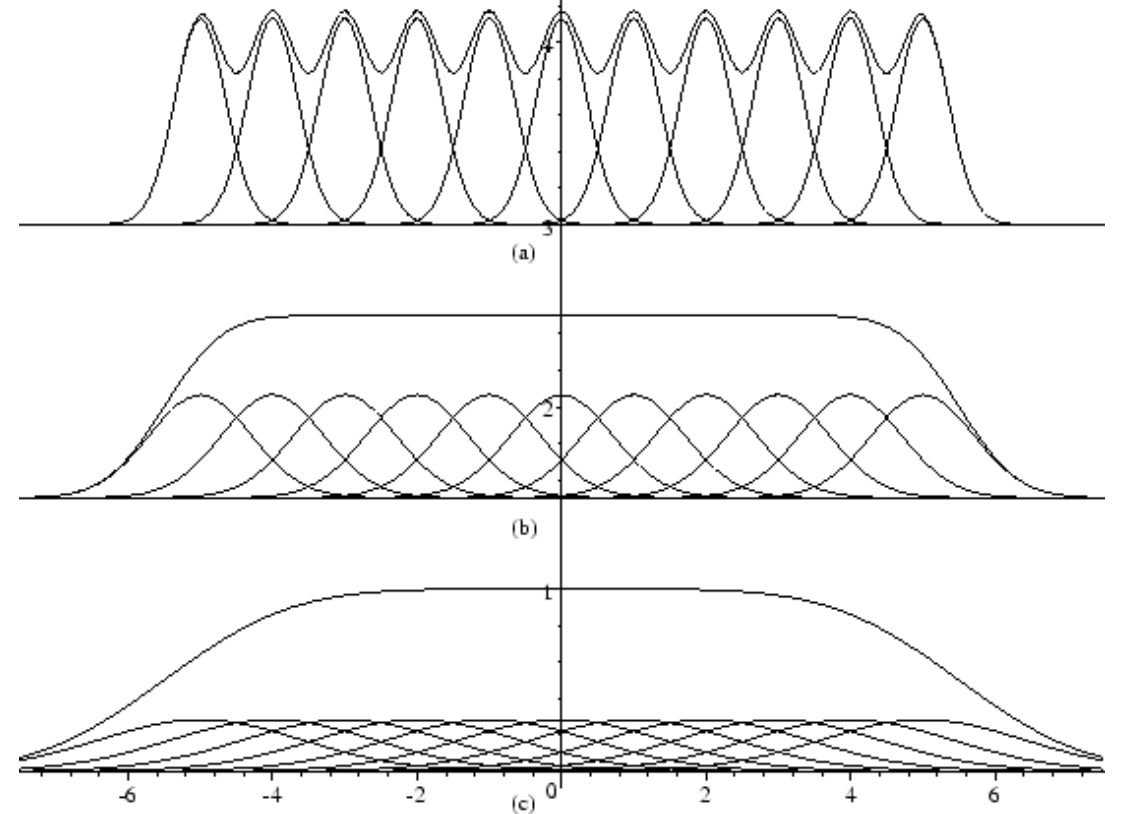
\includegraphics[width=0.8\textwidth]{smoothing.png}
			\caption{a) h=0.5 b) h=1 c) h=2}
			\label{fig:smoothing}
			\end{figure}
			Rysunek \ref{fig:smoothing} pokazuje co może się stać jeśli źle dobierzemy wartość promienia wygładzania. Pokazuje on równoodległe cząstki o tej samej wadze. Obliczona gęstość docelowo powinna przypominać linię ${\rho}$ = 1. Widać natomiast, że w c, gdzie dobraliśmy zbyt duże h linia ta znacząco przewyższa wartość oczekiwaną. Poprawnie dobrane h, do którego winniśmy dążyć, leży gdzieś pomiędzy przykładem a i b.
			
		\subsection{Wzory użytkowe}
			\subsubsection{Gęstość}
			Z równania (\ref{eq:calc_all}) gęstość w dowolnym punkcie możemy obliczyć korzystając ze wzoru \[{\rho}_i=\sum_{j=1}^{N}m_jW(r_{ij},h_j) \label{eq:calc_density} \tag{8}\] 
			\subsubsection{Równanie stanu}
			Jako równanie stanu wykorzystaliśmy zaproponowaną przez Monaghana w [Monaghan J.J. Sph without a tensile instability. J. Comp. Phys., 159:290-311, 1999.] funkcję:
			\[p_i(\rho)=\frac{\rho_0 c_0^2}{\gamma}[(\frac{\rho_i}{\rho_0})^{\gamma} - 1] \label{eq:calc_state} \tag{8}\]
			gdzie ${c_0}$ to prędkość dźwięku przy zadanej gęstości ${\rho_0}$, a ${\gamma}$ ma wartość 7, dzięki czemu płyn jest odporny na ściskanie. $\rho_0$ jest gęstością spoczynkową układu, do której dążyć będą wszystkie obszary gęstości. Łatwo zauważyć iż dzięki podniesieniu ilorazu gęstości do wysokiej potęgi (wskazana wartość wyznaczona została jako optymalna) nawet małe odchylenia gęstości powodować będą duże różnice ciśnienia, co uodparnia układ na ściskanie.
			
			Możliwe jest także użycie prostszego wyrażenia:	
			\[p_i(\rho) = k(\rho_0 - \rho_i) \tag{9}\]
			
			daje ono możliwość symulowania zachowań gazu, ponieważ umożliwia ściskanie w dużo większym stopniu niż ($\ref{eq:calc_state}$).
			
			\subsubsection{Różnica ciśnień}
			Przekształcenia opisane w \cite{Boryczko} pokazują, że skłądową sił pochodząca od ciśnienia, działającą na cząstkę i można zapisać jako: \[\frac{\nabla P_i}{\rho_i} = \sum_j m_j(\frac{P_j}{{\rho_j}^2} + \frac{P_i}{{\rho_i}^2})\nabla W(r_{ij}, h_j) \label{eq:calc_pressure} \tag{9}\] Gdzie ${\nabla}$W to piersza pochoda funkcji wygładzającej po odległości.
			
			\subsubsection{Lepkość}
			Oprócz oczywistego wzoru na lepkość wynikającego bezpośrednio z (\ref{eq:navier-stokes}) istnieje wiele innych modeli lepkości \cite{Boryczko}.
						
			W naszym projekcie wykorzystaliśmy model Monaghana ponieważ dawał zadowalające wyniki i był najmniej złożony obliczeniowo. Składnik ten wyrażony jest wzorem:
			
			\[{\Pi}_{ij} = \frac{-\alpha \mu_{ij} c_{ij} + \beta\mu_{ij}^2}{\rho_{ij}} \label{eq:viscosity_term} \tag{10}\]
	
			gdzie $\alpha$ i $\beta$ są parametrami modelu, a ich wartość zależy od oczekiwanych właściwości symulowanego płynu, $c_{ij} = (c_i + c_j) / 2$ (gdzie $c_i = (\gamma p_i / \rho_i)^\frac{1}{2}$ to prędkość dźwięku w miejscu $r_i$) oraz:
			
			\[{\mu}_{ij} = \left\{
				\begin{array}{l l}
					\frac{(v_i - v_j)\cdot(r_i - r_j)}{h_{ij}(||r_i - r_j||^2 / h_{ij}^2 + \eta^2)} & \quad if{(v_i - v_j)\cdot(r_i - r_j) < 0}  \\ 0 & \quad if{(v_i - v_j)\cdot(r_i - r_j) \geq 0} 
				\end{array} \right.\ \label{eq:mu_factor} \tag{11}\]
				
			Promień wygładzania obliczyć można jako $h_{ij} = (h_i + h_j)/2$, jednakże w naszym przypadku jest on zawsze stały, więc $h_{ij}$ zamienić można na $h$. Ta postać modelu lepkości jest kombinacją tzw. lepkości bulk (liniowa względem $\mu_{ij}$) oraz lepkości von Neumanna-Richtmeyera (kwadratowo zależna od $\mu_{ij}$). Lepkość von Neumanna-Richtmeyera zaproponowana została do symulacji uderzeń w celu zapobiegnięcia zjawisku przenikania się cząstek. 
			

			Jak wykazano w \cite{Lombardi}, wyniki najbliższe rzeczywistości można uzyskać przyjmując $\alpha \approx 0.5, \beta \approx 1.0$ oraz $\eta \approx 0.1$

\section{Cele projektu}
\label{sec:cele}

Bardzo ciężko jest znaleźć w internecie poprawną implementację metody SPH wraz z wizualizacją, działającą w czasie rzeczywistym. W technologii OpenCL, na którą się zdecydowaliśmy, taka implementacja po prostu nie istnieje (lub nam nie udało się jej znaleźć). Rozwój algorytmów opartych o GPGPU jest rzeczą widoczną od stosunkowo niedawna, więc projekt ten jest pracą na swój sposób pionierską mającą pokazać zasadność skorzystania z tej techniki w symulacjach.
		
	Po konsultacji z opiekunem główne założenia projektu zostały określone następująco:
	
	\begin{itemize}
	
		\item Przeprowadzenie wszystkich obliczeń wymaganych do ostatecznego zasymulowania zachowania płynu metodą SPH na wielordzeniowej architekturze przy użyciu zestawu narzędzi OpenCL lub CUDA (zdecydowaliśmy się na OpenCL)
				
		\item Optymalizacja wydajności użytych rozwiązań w celu uzyskania możliwie najlepszego stosunku jakości do płynności animacji (przyjęto, że $\sim 30$ klatek na sekundę jest ograniczeniem dolnym w kwestii płynności animacji)
		
		\item Graficzna prezentacja wyników w czasie rzeczywistym
	
		\item Stworzenie dokumentacji, która będzie zawierała nasze przemyślenia odnośnie tworzonego produktu w celu umożliwienia potencjanemu użytkownikowi rozwoju oprogramowania w przyszłości.
		
	\end{itemize}
	
\section{Zakres funkcjonalności}
	
	Docelowym produktem jest interaktywna aplikacja graficzna wyświetlająca symulację przerwania tamy. Symulacja cieczy powinna spełniać wszystkie cele określone w sekcji \ref{sec:cele}.
	
		Ponadto aplikacja powinna umożliwiać poruszanie się po wirtualnym świecie, dobieranie parametrów symulacji takich jak lepkość czy gęstość cieczy oraz restartowanie symulacji.
	
\section{Opis wykorzystanych technologii}

\subsection{OpenCL}
			Programowanie w OpenCL polega na pisaniu w OpenCL C (języku zbliżonym składniowo do C++99, z pewnymi rozszerzeniami umożliwiającymi łatwiejsze operowanie na wektorach i macierzach) funkcji zwanych jądrami, którym przekazujemy dane z hosta (CPU) które następnie są uruchamiane w olbrzymiej ilości wątków (najczęściej na GPU). Możemy w ten sposób wykonać zdefiniowane w kernelach operacje na różnych zbiorach danych równolegle. 
			
			Należy również z poziomu hosta dobrać odpowiednie parametry wywołania jąder. Jest to operacja bardzo bliska sprzętowi. Istnieje na przykład możliwość, że zły dobór parametrów zamiast uruchomić obliczenia na GPU spowoduje błąd. Należy brać to pod uwagę, szczególnie jeśli jednym z celów pisanej aplikacji jest wieloplatformowość.
			
			OpenCL posłużył nam do implementacji wszystkich algorytmów składających się na metodę SPH. Ideą pracy była próba osiągnięcia maksymalnej wydajności, dzięki wykorzystaniu możliwości paralelizacji wykonywanych obliczeń. Przydatne były także techniki takie jak OpenCL/OpenGL interop, które umożliwiły ominięcie zauważalnie kosztownego kroku odczytu danych z pamięci karty graficznej do pamięci RAM przy wizualizacji, dzięki przechowywaniu wszyskich danych na karcie graficznej. W OpenCL zaimplementowaliśmy algorytmy takie jak sortowanie, wyszukiwanie sąsiadów, podział pudła obliczeniowego czy obliczenia związane z SPH. Pomimo iż wiele z nich można zrealizować na różne sposoby, to wciąż da się je sprowadzić do dużej ilości niezależnych obliczeń.
			
\subsection{Inne}

	\subsubsection*{OpenGL}
			Jest to specyfikacja otwartego i uniwersalnego API do tworzenia grafiki. Ciekawym resultatem uniwersalności bibliotek typu OpenGL i OpenCL jest to, że de facto OpenCL i OpenGL same w sobie są jedynie specyfikacjami API a nie implementacjami. W gestii producentów leży implementacja danego API na dostarczane urządzenie.

\subsubsection*{CLPP}
			 Jest to ogólnodostępna biblioteka do sortowania z wykorzystaniem OpenCL. Wykorzystaliśmy ją w projekcie ponieważ sortowanie było kluczowym elementem algorytmu, a clpp oferowało wysoce zoptymalizowaną, w stosunku do naszej, implementację radix sorta działająca na GPU.

\subsubsection*{GLFW}
			 Jest to jedna z najlżejszych wieloplatformowych bibliotek do tworzenia i obsługi okien, dostępnych w C++. W naszym projekcie klasy Window i InputManager są wrapperami na funkcjonalności GLFW. Ma ona tę wadę, że nie umożliwia łatwego wyświetlania tekstu czy prostych obiektów geometrycznych w oknie tak jak konkurencyjne biblioteki SFML, SDL czy FreeGLUT. 

\subsubsection*{Boost.Signals2}
			 Biblioteka boost jest przez wielu uważana za drugi standard C++, oczywiśćie po libstdc++. Boost.Signals2 udostępnia funkcjonalność sygnałów i slotów, zbliżoną na przykład do systemu eventów w językach takich jak C\#. Została ona wykorzystana do stworzenia globalnego systemu zdarzeń, dzięki któremu trywialnym stało się pisanie mapowania działań użytkownika na funkcje wewnątrz programu. 


\section{Opis realizacji}

	\subsection{Kluczowe elementy stworzonego frameworku}
		\subsubsection{Obsługa OpenGL i okna}
			Klasa OpenGLSystem zajmuje się inicjalizacją okna oraz dostarczaniem informacji na temat kontekstu OpenGL, które są niezbędne do poprawnej inicjalizacji urządzenia OpenCL. Istnieje bowiem możliwość, że system OpenCL zostałby zainicjalizowany na urządzeniu innym niż OpenGL przez co niemożliwa byłaby komunikacja z wykorzystaniem OpenCL\\OpenGL interop.
			
			Klasa Window oraz klasa InputManager stanowią wrapper na funkcjonalności biblioteki GLFW. Umożliwiają one inicjalizację okna oraz obsługę zdarzeń wywołanych przez użytkownika takich jak naciśnięcie klawisza czy ruch myszką. 
			
		\subsubsection{Obsługa OpenCL}
			Klasa OpenCLSystem stanowi lekki wrapper na wszystkie konieczne funkcje OpenCL takie jak:
			\begin{itemize}
				\item Wykrywanie urządzenia, na którym jest zainicjalizowany OpenGL
				\item Tworzenie kontekstu OpenCL
				\item Czytanie i budowanie jąder OpenCL
			\end{itemize}
			W kodzie funkcjie OpenCL przeważnie są wywoływane bezpośrednio, jako że API OpenCL jest klasycznym API w języku C, które przechowuje wewnętrznie swój własny stan.
			
		\subsubsection{Obsługa zdarzeń}
			Klasa EventManager wraz z interfejsem IEventData oraz typem wyliczeniowym EventType stanowią trzon systemu zdarzeń w stworzonym frameworku. Ideą tego systemu jest to, że każda klasa może się zarejestrować na odbiór pewnego rodzaju eventów oraz sama wysłać event do systemu. Klasa EventManager jest przez to globalna dla całej aplikacji. W każdej klatce zdarzenia, które wystąpiły są wysyłane do opowiednich odbiorców.
			
			Dzięki tej klasie osiągamy inwersję zależności (dependency inversion). Poszczególne obiekty systemu nie muszę wiedzieć o żadnych innych obiektach. Chcąc poinformować, że zaszło jakieś zdarzenie lub chcąc wysłać jakąś wiadomość do systemu jedyne co obiekty muszą posiadać to referencję do EventManager'a. To on zajmuje się dystrybucją wiadomości do zainteresowanych odbiorców.
		 
		\subsubsection{Model aktorów złożonych z komponentów}
		
			W każdej grze istnieje koncepja aktorów (zwanych czasami obiektami gry (and. game object)), które mogą wykonywać jakieś akcje w czasie, posiadają logikę rysowania, przechowują swój stan i położenie. Klasyczne podejście do budowy tego typu obiektów - wszystko w jednej klasie - łamie SRP (Single Responsibility Principle). Postanowiliśmy więc wykorzystać model zwany CBSE (Component-Based Software Engineering) do reprezentacji aktorów. 
			
			Każdy aktor składa się z wielu komponentów definujących takie rzeczy jak logikę, sposób rysowania, przemieszczenie w przestrzeni. Mogą też istnieć specyficzne komponenty takie jak komponent kamery. Jako, że każdy komponent zajmuje się swoją własną dziedziną nie jest łamane SRP i system staje się znacząco bardziej skalowalny. 
			
			Przykładem zastosowania tego modelu są klasy WaterLogicComponent, WaterModelComponent oraz WaterRenderComponent - każda z nich zajmuje się dostarczeniem jednej funkcjonalności. WaterLogiComponent zawiera logikę OpenCL, która porusza modelem płynu zdefiniowanym i zainicjalizowanym w WaterModelComponent. WaterRenderComponent natomiast komunikuje się z WaterModelComponent w celu wyświetlenia modelu cieczy na ekranie. Łatwym byłoby stworzenie innego sposoby renderowania czy innego zachowania cieczy (co było wykonywane w pierwszych iteracjach) i polegałoby tylko na podmianie tych, raczej lekkich, komponentów.
			
		\subsubsection{Wykorzystanie C++11}
		
		Pisząc kod stosowaliśmy się do idiomu C++ RAII (Resource Acquisition Is Initialization). W całym kodzie słowo kluczowe "delete" praktycznie nie występuje ponieważ wszystkie zmienne są inicjalizowane w taki sposób, aby kiedy nie są potrzebne same się usuwały. Wykorzystujemy do tego takie dodatki w C++11 jak shared\_ptr, unique\_ptr czy std::array zamist zwykłych wskaźników i wskaźników na tablice. Korzystamy też z nowowprowadzonych lambd oraz słowa kluczowego auto.
		
	\subsection{Kluczowe elementy implementacji metody SPH}
		
		Nasza implementacja metody SPH składa się z 9 jąder i wykorzystujemy 10 globalnych buforów. Dodatkowo korzystamy z biblioteki clpp, która dostarcza nam optymalnych implementacji sortowań na kartę graficzną algorytmem Radix Sort.
		
		\noindent Przebieg algorytmu wygląda następująco:
			\begin{enumerate}
			\item{Znajdowanie sąsiadów cel}
			
				Dane pudło obliczeniowe jest logicznie dzielone na pewną ilość sąsiadujących, sześciennych cel o boku równym dwukrotności promienia odcięcia. Każda taka cela jest logicznie dzielona na 8 podcel. Dla każdej podceli musimy znać listę sąsiadujących cel (łącznie 8 w tym cela w której znajduje się podcela).
			\item{Przypisywanie cząstek do cel}
			
				Dla każdej cząstki obliczemy w której znajduje się celi. Jako, że cząstki w buforze "positions" są posortowane po numerze cząstki, to wynikiem tej operacji jest lista par (numer cząstki, numer celi) posortowana po numerze cząstki.
			\item{Sortowanie cząstek po numerze celi}
			
				Naszym celem jest rozumowanie o cząstkach w kontekście cel w których się znajdują. Dlatego sortujemy stworzoną w poprzednim kroku listę par po numerze celi.
			\item{Sortowanie pozycji i prędkości}
			
				Aby móc łatwiej rozumować o cząstkach, sortujemy pozycje i prędkości w taki sam sposób jak została posortowana w poprzednim kroku lista par (numer cząstki, numer celi).
			\item{Odnajdywanie indeksów w posortowanych tabelach}
			
				Brakuje nam informacji o tym gdzie w posortowanych tablicach zaczynają i kończą się informację o danej celi. Odnajdujemy odpowiednie indeksy początka i końca informacji o celach co też daje nam możliwość
				
			\item{Znajdowanie sąsiadów cząstek}
			
				Kluczowym elementem całego algorytmu, do którego dążą wszystkie poprzednie kroki, jest znalezienie dla każdej cząstki ustalonej liczby sąsiadów. Badania pokazały 55 sąsiadów w zupełności wystarcza do realistycznej symulacji. Nie trzeba za każdym razem znajdować wszystkich w odległości mniejszej niż promień odcięcia. Dzięki informacjom uzyskanym w krokach 1, 4 i 5 możemy znacząco ograniczyć pole przeszukiwań, szukając tylko w najbliższych celach.
			\item{Obliczenie gęstości i ciśnienia}
			
				Korzystając ze wzorów danych w metodzie SPH obliczamy gęstość oraz ciśnienie.
			\item{Obliczenie przyspieszenia cząstek}
			
				Korzystając ze wzorów danych w metodzie SPH obliczamy przyspieszenie cząstek.
			\item{Krok czasowy}
			
				Przemieszczamy cząstki, korzystając z prostych równań fizycznych.
				
			\end{enumerate}
			
			Do implementacji zostały wykorzystane następujące struktury danych:
			\ \\
			\ \\
			\begin{tabular}{| p{\dimexpr 0.27\linewidth-2\tabcolsep} | p{\dimexpr 0.25\linewidth-2\tabcolsep} | p{\dimexpr 0.48\linewidth-2\tabcolsep} |}
				\hline
					Nazwa bufora & Typ i rozmiar & Opis zastosowania \\
				\hline
					position & float4[ilość cząstek] & Pozycje cząstek - bufor ten jest współdzielony z OpenGL i jest wykorzystywany do wizualizacji cząstek. \\
				\hline
					velocity & float4[ilość cząstek] & Prędkości cząstek \\
				\hline
					acceleration & float4[ilość cząstek] & Wektor przyspieszenia dla każdej cząstki\\
				\hline
					grid\_cell\_index & int[ilość cel] & Indeksy początków danych dla każdej celi w tablicy voxel\_particle \\
				\hline
					voxel\_particle & int2[ilość cząstek] & Mapa zawierająca przypisania cząstek do cel \\ 
				\hline
					sorted\_position & float4[ilość cząstek] & Pozycje cząstek posortowane jak voxel\_particle\\
				\hline
					sorted\_velocity & float4[ilość cząstek] & Prędkości cząstek posortowane jak voxel\_particle\\
				\hline
					density\_and\_pressure & float2[ilość cząstek] & Gęstość i ciśnienie dla każdej cząstki\\
				\hline
					neighbour\_map & int[neighbours\_to\_find ${\cdot}$ ilość cząstek] & Mapa sąsiadów każdej cząstki\\
				\hline
					voxel\_neighbour\_map & int[64 ${\cdot}$ ilość cel] & Sąsiedzi dla każdej celi \\
				\hline
			\end{tabular}



\section{Organizacja pracy}

\subsubsection*{Dawid Romanowski} 
		
		\begin{itemize}
		
			\item w ramach dokumentacji technicznej
			
				\begin{itemize}
				
					\item Opis OpenCL
					\item Struktura projektu
					\item Sposób implementacji metody SPH
					\item Sposób implementacji wizualizacji metody SPH
					\item Opis wykorzystanych zewnętrznych bibliotek
				
				\end{itemize}
			
			\item w ramach dokumentacji procesowej
			
				\begin{itemize}
				
					\item Pomoc przy formułowaniu celów pracy
					\item Zapisywanie minutek w trakcie spotkań
				
				\end{itemize}
			
			\item w ramach dokumentacji użytkownika
			
				\begin{itemize}
				
					\item Opis metody SPH - od wstępu do opisu funkcji wygładzających włącznie
					
					\item GPGPU i OpenCL
					
					\item Korzystanie z programu wraz z zrzutami ekranu
				
				\end{itemize}
			
			\item zaplanowanie oraz implementacja finalnej architektury systemu
			
			\item implementacja kerneli związanych z wyszukiwaniem sąsiadów
			
			\item zarządzanie plikami CMake w celu zapewnienia poprawnej kompilacji i linkowania aplikacji w systemach z rodziny debian (Linux Mint, Ubuntu).
		
		\end{itemize}
		
	\subsubsection*{Wojciech Czarny} 
		
		\begin{itemize}
			
			\item w ramach dokumentacji procesowej
			
				\begin{itemize}
				
					\item Wizja projektu, cel projektu, opisy problemu i użytkowników, wymagania.
					
					\item Dokumentacja przebiegu pracy, kamieni milowych, minutek.
					
					\item Sformułowanie podsumowania, określenie stopnia realizacji założeń i dalszych kierunków rozwoju, udokumentowanie użytych narzędzi oraz podziału prac
				
				\end{itemize}
			
			\item w ramach dokumentacji użytkownika
			
				\begin{itemize}
				
					\item Opis metody SPH - część wzorów użytkowych, 
					
					\item GPGPU i OpenCL
				
				\end{itemize}
				
			
			\item stworzenie prototypu modułu graficznego i obliczeniowego
			
			\item wsparcie przy implementacji finalnej architektury systemu
			
			\item implementacja kerneli związanych z zarządzaniem danymi oraz kerneli realizujących obliczenia metody SPH
					
			\item zarządzanie plikami CMake w celu zapewnienia poprawnej kompilacji i linkowania aplikacji w systemie Windows 8.1
		
		\end{itemize}

\section{Wyniki projektu}

Udało się stworzyć aplikację będącą PoC (Proof of Concept, ang. dowód koncepcji) badanego problemu. Aplikacja ta przeprowadza symulację zachowania płynu przy użyciu metody SPH zaimplementowanej jako seria jąder OpenCL. Wyniki przeprowadzanej symulacji wizualizowane są w czasie rzeczywistym przy użyciu OpenGL. Płynność uzyskanej animacji zależy oczywiście od ilości symulowanych cząstek, jednak zdaniem naszym i klienta jest ona zadowalająca. Przy ilościach cząstek rzędu milion uzyskujemy ponad 30 fps.
		
		Poniższe elementy nie zostały zrealizowane w pełni bądź pominięte, głównie z powodu braku czasu. Nie są to elementy niezbędne do poprawnego działania projektu, jednakże ich realizacja bardzo pomogłaby w dalszym rozwoju stworzonego oprogramowania.
		
		\begin{itemize}
		
			\item Stworzenie przejrzystego interfejsu użytkownika dostarczającego informacje potrzebne do debugowania kodu. Okazało się, że poprawna implementacja wszystkich elementów logiki aplikacji jest niewystarczająca do poprawnego działania symulacji, kluczowym jest także dobór odpowiednich stałych parametrów równań. Pomimo iż udało nam się dobrać przykładową poprawną parametryzację, zmiana dowolnej stałej wymaga dostosowania wszystkich pozostałych, co bez znajomości informacji takich jak np. maksymalne/średnie/minimalne ciśnienie występujące w chwili obecnej w układzie jest niezwykle uciążliwe i trudne. Kluczowym jest więc stworzenie modułu odpowiedzialnego za wyciąganie takich danych z pamięci karty graficznej, a następnie wyświetlanie ich w postaci tekstu w oknie graficznym aplikacji. Do osiągnięcia tego celu zaleca się wymianę biblioteki odpowiedzialnej za zarządzanie oknem (w chwili obecnej GLFW) na bibliotekę o wyższym poziomie abstrakcji (np. SDL, SFML), co umożliwiłoby zarówno zachowanie funkcjonalności zarządzania oknem graficznym, jak i łatwą integrację wyświetlania tekstu.
			
			\item Podpięcie odpowiednich zdarzeń związanych z wprowadzaniem wejścia z klawiatury do logiki odpowiedzialnej za zmianę stałych parametrów równań. Umożliwiłoby to zmianę stałych w trakcie wykonywania symulacji i jednoczesną obserwację ich poprawności. Dzięki temu możliwe byłoby dużo łatwiejsze dobranie poprawnych parametrów poprzez bezpośrednie badanie ich wpływu na zachowanie symulowanego płynu.
			
			\item Możliwa jest także wymiana sposobu liczenia składowej lepkości przy obliczaniu przyspieszenia cząstki. Obecny sposób może nie dawać najbliższych rzeczywistości rezultatów wizualnych.
			
			\item W chwili obecnej możliwe jest przeprowadzenie symulacji w prostopadłościennym pudle obliczeniowym poprzez umieszczenie w nim prostopadłościennej ściany równo oddalonych od siebie cząstek płynu. Następnie pod wpływem grawitacji i sił oddziaływań między nimi zaczynają się one przemieszczać w obrębie pudła. Aby zaobserwować bardziej skomplikowane zjawiska i właściwości obserwowanego układu należałoby zaimplementować moduł odpowiedzialny za tworzenie i zarządzanie prostymi bryłami kolizyjnymi. Bryły pełniłyby wewnątrz pudła tą samą funkcję co ściany pudła, jednakże składając je w bardziej skomplikowane kształty można by zaobserwować zjawiska takie jak opływanie przeszkody z dwóch stron przez cząstki płynu oraz wydostawanie się cząstek płynu z naczynia przez otwór.
			
			\item Możliwa jest dalsza optymalizacja obliczeń w celu uzyskania mniejszych wymagań ze strony sprzętu, co pozwoliłoby na zwiększenie dopuszczalnej ilości cząstek biorących udział w symulacji lub zwiększyłoby zakres sprzętu, na którym można przeprowadzić symulację. M.in. należałoby rozważyć które bloki instrukcji wykonywanych sekwencyjnie w kernelach OpenCL można zastąpić przez wykonanie ich za pomocą grup lokalnych.
		\end{itemize}

\nocite{OpenCLProgrammingGuide, GameCodingComplete, CLPP, SPHWebinar, Lucy, MonLat, Boryczko, Lombardi}
\bibliography{bibliografia}

\end{document}

